After the discovery of the Higgs boson at the LHC, and the first exploration of the couplings of the new particle at the run 1 and 2, achieving an overall precision at the level of ten percent, one of the main goal of Higgs studies at the HL-LHC or HE-LHC will be to push such limits to a percent level. In this section we study the projected precision that would be possible at such high luminosity and high energy extensions of the LHC from a global fit to modifications of the different single Higgs couplings.
Other important goals of the Higgs physics program at the HL/HE-LHC, such as extending/complementing the onshell studies with the study of differential distributions, or getting access to the Higgs trilinear coupling will be covered in other parts of this document.

Many explorations of deviation in Higgs couplings in the context of future proposed experiments are typically presented in the so called $\kappa$ framework~\cite{LHCHiggsCrossSectionWorkingGroup:2012nn,Heinemeyer:2013tqa}. In this phenomenological formalism one defines scaling factors, denoted $\kappa_i$, such that the production cross sections and decays of the Higgs boson involving the SM particle $i$, scale as $\kappa_i^2$.
This is indeed a helpful approach to quantify the precision in Higgs measurements. However, it lacks robustness from the theory point of view, as it cannot be extended at NLO and, in its more general form, misses correlations derived from well established symmetry principles. A more robust[/reliable] exploration of deformations in Higgs couplings can be performed within the formalism of effective field theories. In this section we consider the general parameterization provided by non-linear Higgs effective field theory. As explained, in section~\ref{sec:kappavsEFT}, as long as we restrict to the LO effective Lagrangian and one focuses only on deviations on Higgs couplings, it is possible to connect the results of this formalism to those from the $\kappa$ framework.
We refer the reader to section~\ref{sec:kappavsEFT} for the introduction of the non-linear Higgs effective Lagrangian and its connection with the $\kappa$ formalism. Throughout this section we will present the expected sensitivities to deviations on the Higgs couplings at the HL/HE-LHC, and compare with the recent results obtained using current data from \cite{deBlas:2018tjm}. A more general analysis going beyond pure modifications of Higgs couplings, allowing also for new physics also in EW interactions, and combining the results of the Higgs fit with those from EW precision observables and diboson measurements will be presented in section~\ref{sec8:fit}. Such effect may become relevant once the precision on the Higgs measurements goes below the threshold were the sensitivity to other EW interactions is comparable to that from current EW precision tests.

In what follows we detail the fit procedure, the HL/HE-LHC projections used in our analysis, as well as the corresponding references for the analysis to current experimental data. We then present the results of the fit to the projected HL/HE-LHC uncertainties for the two formalisms mentioned above. We also translate the results from the fit to the HL/HE-LHC data in the EFT formalism in terms of composite Higgs scenarios. These are presented and discussed in section~\ref{sec9:CHM}.
\subsubsection{The fit to HL/HE-LHC Higgs precision data}

The fits presented in this section have been performed using the {\tt HEPfit} package~\cite{hepfit,hepfitsite}, and following a statistical Bayesian approach. The prior for the different model parameters both in the EFT and in the $\kappa$ framework are taken as flat, centered around the SM solution, and restricting the ranges to avoid other solutions present due to the parametrization invariances of the different formalisms.
Since no sensitivity to the $H\to c\bar{c}$ channel at the HL/HE-LHC has been reported yet we fix the corresponding parameters controlling the $Hc\bar c$ interactions to their SM values ($c_c,\kappa_c=1$).~\footnote{See ~\cite{deBlas:2018tjm} for a discussion of the multiplicities of the different solutions in the fit as well as the effect of letting the charm coupling float in the fits in absence of a significant direct constraint.}

To assess the sensitivity to deviations from the SM, we assume the future measurements are SM-like and include them in the likelihood of the fit assuming Gaussian distributions with standard deviations given by the corresponding experimental uncertainty. 

The analysis of current constraint has been taken directly from~\cite{deBlas:2018tjm}, it is based on the experimental data from~\cite{Aad:2014eha,Aaboud:2018xdt,Khachatryan:2014ira,CMS:2017rli,Aad:2014eva,Aaboud:2017vzb,Khachatryan:2014jba,Sirunyan:2017exp,Aaboud:2017jvq,Sirunyan:2018shy,ATLAS:2014aga,Aad:2015ona,ATLAS:2016gld,Chatrchyan:2013iaa,Sirunyan:2018egh,Aaboud:2017jvq,Sirunyan:2018shy,ATLAS-CONF-2018-004,Aad:2014xzb,Aaboud:2017rss,Chatrchyan:2013zna,CMS:2016mmc,Aad:2015gra,Aaboud:2017xsd,Khachatryan:2014qaa,Sirunyan:2018mvw,Sirunyan:2018ygk,Sirunyan:2017elk,Aad:2015vsa,Aaboud:2017jvq,Chatrchyan:2014nva,Sirunyan:2017khh,Sirunyan:2018shy,Khachatryan:2016vau,Aaboud:2017ojs,Khachatryan:2016vau,CMS-PAS-HIG-17-019,Aad:2015gba,Aaboud:2017uhw,Chatrchyan:2013vaa,CMS-PAS-HIG-17-007,Aaltonen:2013ipa,Abazov:2013gmz}. 
For the HL-LHC fits we use {\bf [We will use when available]} the corresponding ATLAS and CMS projections presented in section~\ref{???} of this document.  For the systematics and theory uncertainties we use the 2 possible scenarios presented in section~\ref{???}: S1, for which the systematics are kept as in current values, and S2, where experimental systematics are reduced with the luminosity and theory errors are reduced.
%
Finally, we use our ``naive'' estimates for the HE-LHC uncertainties, derived from the
detailed HL-LHC projection by scaling the statistical uncertainties according with the changes in the production cross section going from 14 TeV to 27 TeV, as well as the different luminosities (3 ab$^{-1}$ for the HL-LHC and 15 ab$^{-1}$ in the HE-LHC).
Other experimental and theory uncertainties are kept as in the HL-LHC case, and we use the same S1 and S2 scenarios. To be conservative, no further scaling with the HE-LHC luminosity is applied in the scenario S2, i.e.~it is kept as in the HL-LHC estimates. 
\subsubsection{Results}
{\bf [PRELIMINARY: Based on preliminary CMS numbers from July + Our own guesstimates for HELHC (explained above). 
To be updated when the final experimental projections are available. Conclusions may therefore change.]}\\

In Table~\ref{tab:projection.ci} we show the results of the fit for the different scenarios discussed above for the non-linear Higgs effective Lagrangian. The numbers reported for the HE-LHC are obtained assuming the HL-LHC precision on the Higgs coupling is available at that time. No form of correlation between the HL-LHC and HE-LHC estimates is included, and therefore the 
results may be too optimistic. We also show the same results in Figure~\ref{fig:projection.ci}, where we also indicate the bound obtained
at the HE-LHC alone. The analogous results for the fit using the $\kappa$ formalism are presented in Table~\ref{fig:projection.kappai} and Figure~\ref{fig:projection.kappai}. To make the comparison between the 2 approaches within the same theoretical grounds, we assume custodial symmetry as well as the absence of extra exotic decays of the Higgs in the $\kappa$ fit.
Focusing our attention on the HL-LHC, and taking the conservative S1 scenario as the reference, we observe an improvement on the knowledge of Higgs coupling of at least a factor of 2-3 with respect to current experimental limits. The improvement is more notorious for channels that benefit from very high statistics, such as the $H\to \mu^+ \mu^-$ channel, with a precision almost $6$ times better than in the current fit. Further progress is expected once we include the HE-LHC numbers, getting close to the $1\%$ level of precision for the Higgs couplings to vector bosons and $\tau$ leptons, assuming theory and systematic uncertainties can be kept under control at the same level at the HL-LHC.  One must be careful with the interpretation of these results though, since they implicitly assume only modifications in the Higgs couplings with respect to the SM or, in other words, that any other interaction entering on the relevant Higgs processes is known to be SM-like with infinite precision. At the level of precision we observe, close to the $1\%$, this may not be a justified assumption given current bounds on other electroweak interactions that could modify, e.g.~VBF or VH associated production. This comment applies even more for the uncertainties obtained assuming the reduced theory and systematic uncertainties which, in particular, predict a subpercent precision for the Higgs coupling to vector bosons. We believe this to be too aggressive and that a realistic assessment of the HE-LHC uncertainties requires an equally realistic study of the experimental precisions at that machine, as well as the results of a full global fit combining Higgs data with other relevant observables of the EW sector. We refer to section~\ref{sec8} for more details in this regard.

\begin{table}[ht!]
\begin{center}
\begin{tabular}{ |c||c|c|c|c|c|}
  \hline
  & Current limits~\cite{deBlas:2018tjm}  & HL-LHC S1 & HL-LHC S2 & HE-LHC S1&HE-LHC S2 \\
  \hline
   $c_{V}$&$1.01\pm0.06$ &$\pm 0.021$&$\pm 0.015$&$\pm 0.013$&$\pm 0.008$\\
  $c_{t}$&$1.04^{+0.09}_{-0.1}$&$\pm 0.049$&$\pm 0.028$&$\pm 0.031$&$\pm 0.016$\\
  $c_{b}$&$0.95\pm0.13$ &$\pm 0.046$&$\pm 0.034$&$\pm 0.03$&$\pm 0.02$ \\
  $c_{\tau}$&$1.02\pm 0.1$ &$\pm 0.027$&$\pm 0.02$& $\pm 0.017$&$\pm 0.011$\\
  $c_{\mu}$&$0.58^{+0.4}_{-0.38} $ &$\pm 0.069$&$\pm 0.052$& $\pm 0.035$&$\pm 0.02$\\
  $c_{g}$&$-0.01^{+0.08}_{-0.07} $ &$\pm 0.044$&$\pm 0.025$& $\pm 0.028$&$\pm 0.14$\\
  $c_{\gamma}$ &$0.05\pm0.2 $&$\pm 0.081$&$\pm 0.055$&$\pm 0.051$&$\pm 0.032$\\
\hline
\end{tabular}
\caption{Current and future constraints on $c_{i}$ as shown in Figure~\ref{fig:projection.ci}.}\label{tab:projection.ci}
\end{center}
\end{table}
%
\begin{figure}[ht]
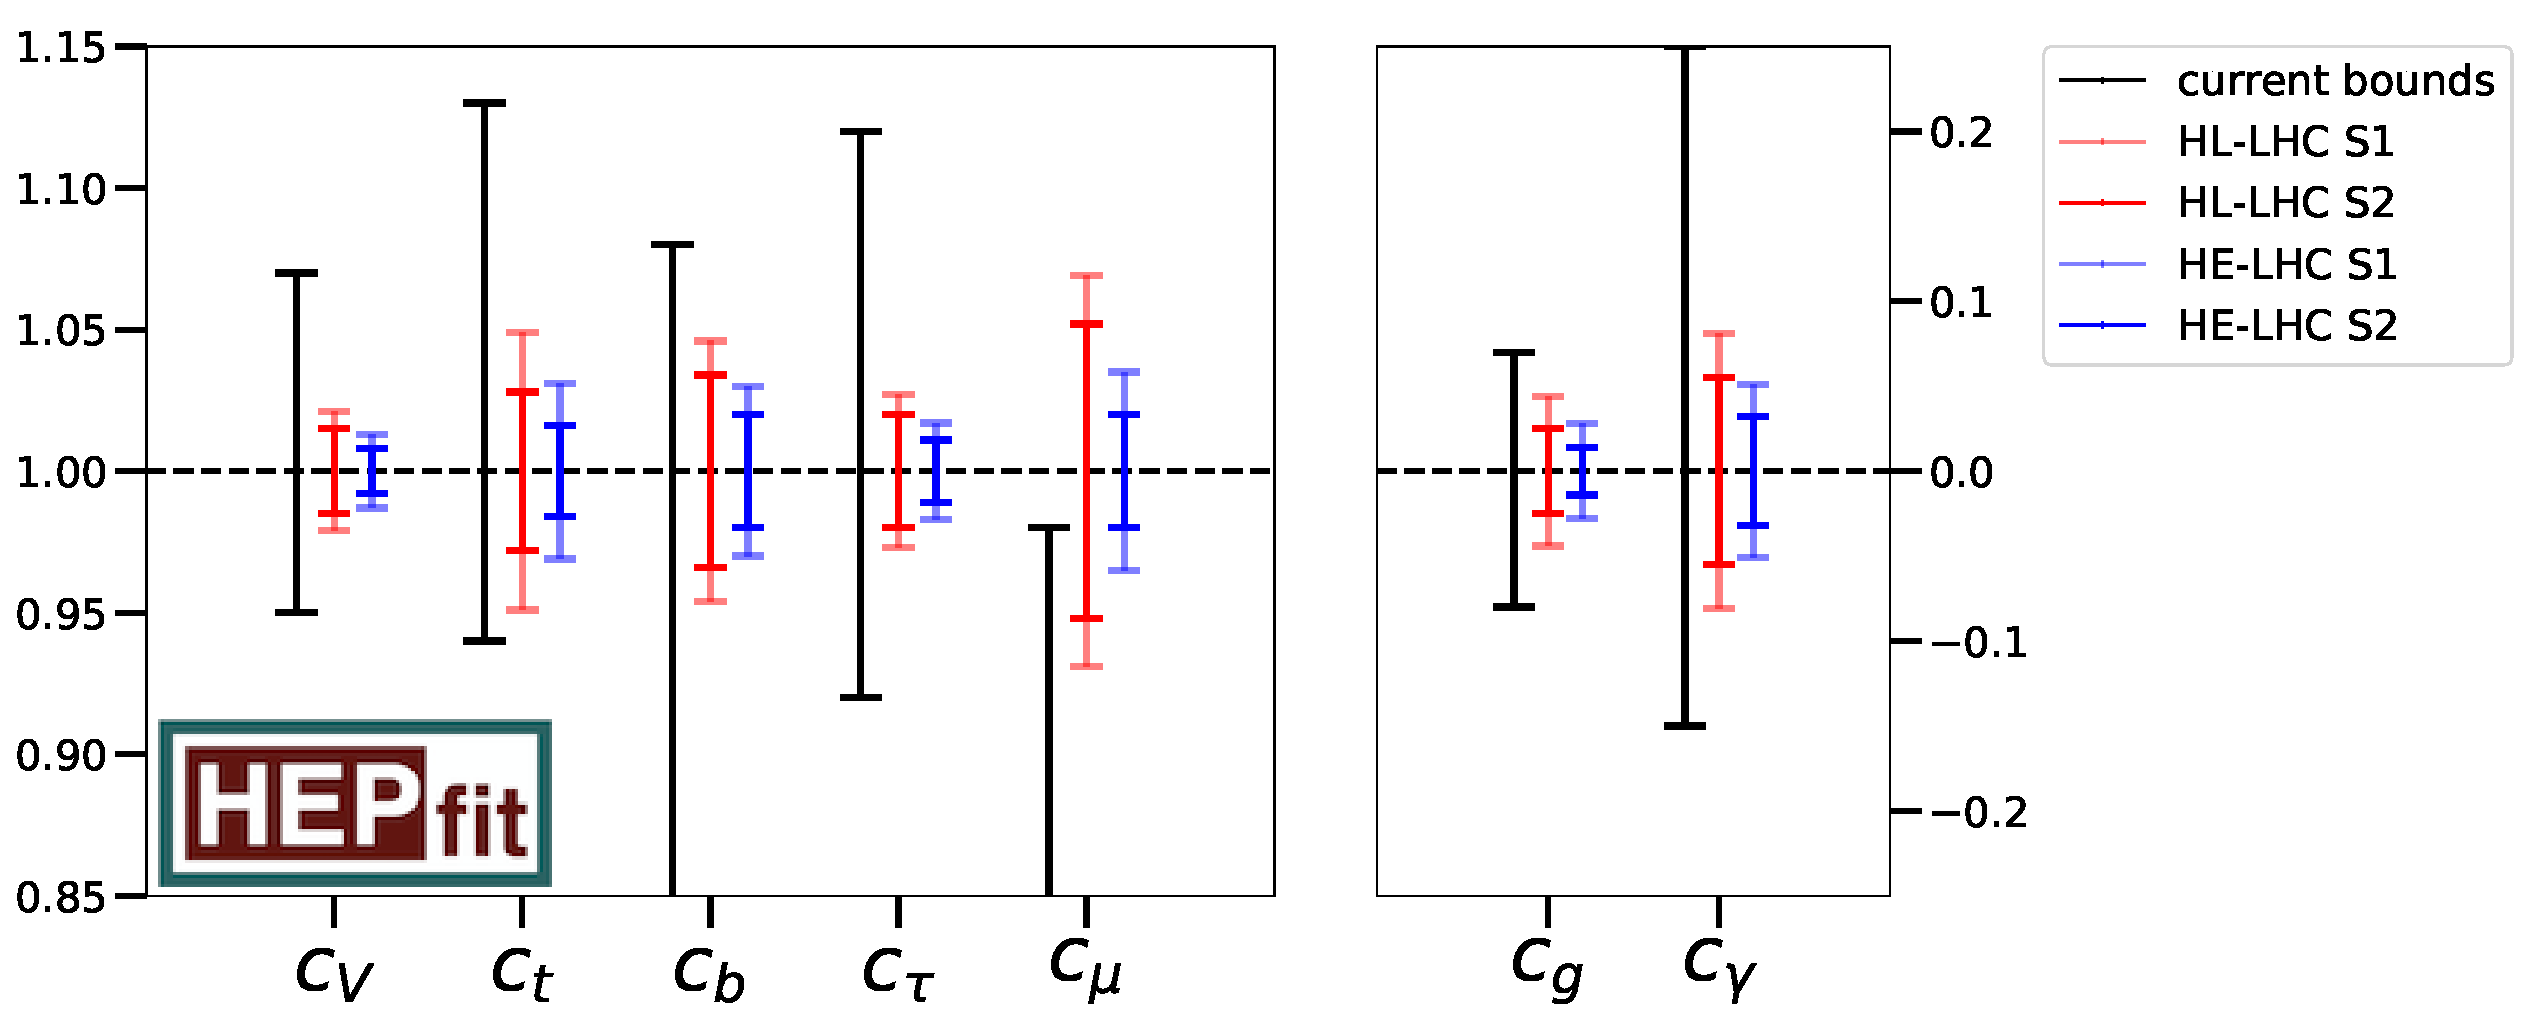
\includegraphics[width=\textwidth]{\main/section2/plots/fit_summary_ci.pdf}
\caption{Current and future constraints on $c_{i}$. The left line of each coupling is the current bound of~\cite{deBlas:2018tjm}. The central line is the projection to the HL-LHC with scenario 1 in light red and scenario 2 in dark red. The right line is the projection to HE-LHC (including HL) with scenario 1 in light blue and scenario 2 in dark blue.}\label{fig:projection.ci}
\end{figure}

\begin{table}[ht!]
\begin{center}
\begin{tabular}{ |c||c|c|c|c|c|}
  \hline
  & Current limits~\cite{deBlas:2018tjm}  & HL-LHC S1 & HL-LHC S2 & HE-LHC S1&HE-LHC S2 \\
  \hline
   $\kappa_{V}$&$1.01\pm0.06$ &$\pm 0.021$&$\pm 0.015$&$\pm 0.013$&$\pm 0.008$\\
  $\kappa_{t}$&$1.04^{+0.09}_{-0.1}$&$\pm 0.049$&$\pm 0.028$&$\pm 0.031$&$\pm 0.016$\\
  $\kappa_{b}$&$0.94\pm 0.13$ &$\pm 0.046$&$\pm 0.034$&$\pm 0.03$&$\pm 0.02$ \\
  $\kappa_{\tau}$&$1.0\pm 0.1$ &$\pm 0.027$&$\pm 0.02$& $\pm 0.017$&$\pm 0.011$\\
  $\kappa_{\mu}$&$0.58^{+0.4}_{-0.38} $ &$\pm 0.069$&$\pm 0.052$& $\pm 0.035$&$\pm 0.02$\\
  $\kappa_{g}$&$1.02^{+0.08}_{-0.07} $ &$\pm 0.035$&$\pm 0.022$& $\pm 0.024$&$\pm 0.13$\\
  $\kappa_{\gamma}$ &$0.97\pm 0.07 $&$\pm 0.028$&$\pm 0.02$&$\pm 0.017$&$\pm 0.011$\\
\hline
\end{tabular}
\caption{Current and future constraints on $\kappa_{i}$ as shown in Figure~\ref{fig:projection.kappai}.}\label{tab:projection.kappai}
\end{center}
\end{table}
%
\begin{figure}[ht]
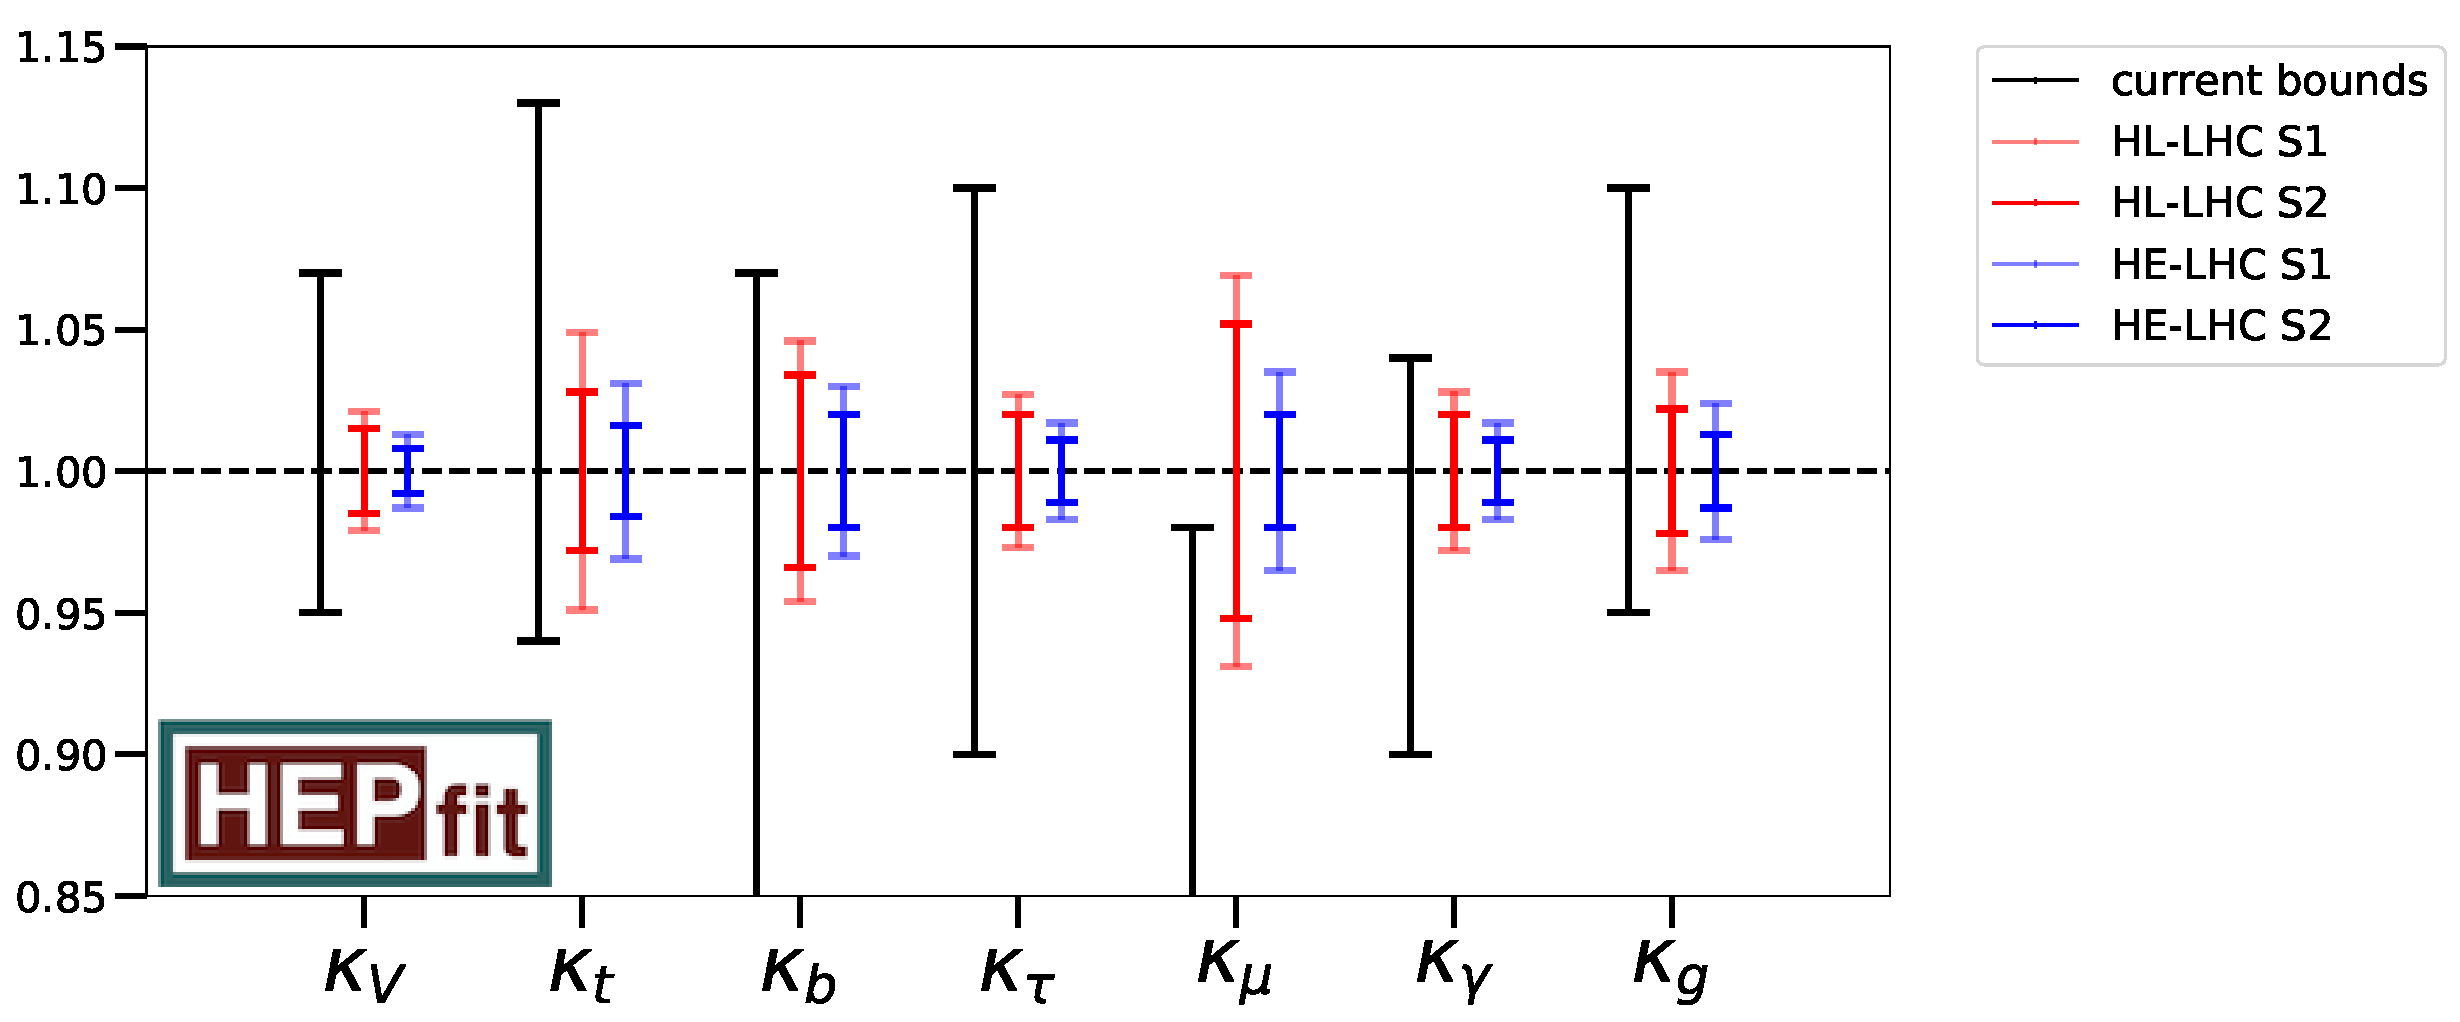
\includegraphics[width=\textwidth]{\main/section2/plots/fit_summary_kappai.pdf}
\caption{Current and future constraints on $\kappa_{i}$. The left line of each $\kappa$ is the current bound of~\cite{deBlas:2018tjm}. The central line is the projection to the HL-LHC with scenario 1 in light red and scenario 2 in dark red. The right line is the projection to HE-LHC (including HL) with scenario 1 in light blue and scenario 2 in dark blue.}\label{fig:projection.kappai}
\end{figure}
